\documentclass{standalone}
\usepackage{tikz}
\usepackage{tikz-qtree}
\usepackage[makeroom]{cancel}
\usetikzlibrary{fit}


\begin{document} 
	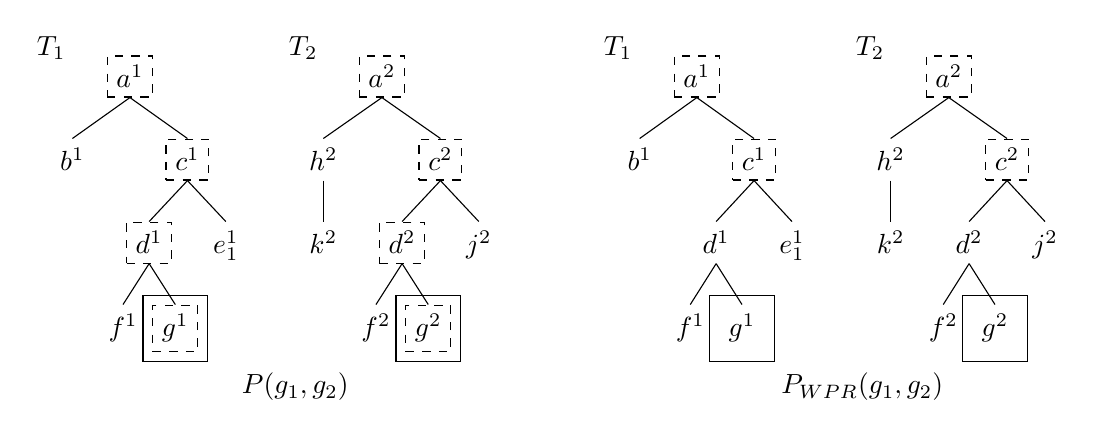
\begin{tikzpicture}[]

		    \node (x) at (-1,0.5) {$T_1$};
		    \node (p1) at (2.1,-3.8) {$P(g_1,g_2)$};
		    \Tree [.\node[draw,dashed]{$a^1$};
		            [.$b^1$ ] 
		            [.\node[draw,dashed]{$c^1$}; 
		                [.\node[draw,dashed]{$d^1$}; 
		                	[.$f^1$ ]
		                	[.\node(g)[draw,dashed]{$g^1$}; ]
		                ]
		                [.$e_1^1$ ] 
		            ]
		          ]
		    \node[draw,fit=(g)]{};
	    

	    \begin{scope}[xshift=3.2cm]
		    \node (y) at (-1,0.5) {$T_2$} ;
		    \Tree [.\node[draw,dashed]{$a^2$};
		            [.$h^2$ 
		            	[.$k^2$ ]
		            ] 
		            [.\node[draw,dashed]{$c^2$}; 
		                [.\node[draw,dashed]{$d^2$}; 
		                	[.$f^2$ ]
		                	[.\node(g)[draw,dashed]{$g^2$}; ]
		                ]
		                [.$j^2$ ] 
		            ]
		          ]
		    \node[draw,fit=(g)]{};
	    \end{scope}


		\begin{scope}[xshift=7.2cm]
			\node (p1) at (2.1,-3.8) {$P_{WPR}(g_1,g_2)$};
		    \node (x) at (-1,0.5) {$T_1$};
		    \Tree [.\node[draw,dashed]{$a^1$};
		            [.$b^1$ ] 
		            [.\node[draw,dashed]{$c^1$}; 
		                [.$d^1$ 
		                	[.$f^1$ ]
		                	[.\node(g){$g^1$}; ]
		                ]
		                [.$e_1^1$ ] 
		            ]
		          ]	
		    \node[draw,fit=(g)]{};
		\end{scope}


		\begin{scope}[xshift=10.4cm]
		    \node (y) at (-1,0.5) {$T_2$} ;
		    \Tree [.\node[draw,dashed]{$a^2$};
		            [.$h^2$ 
		            	[.$k^2$ ]
		            ] 
		            [.\node[draw,dashed]{$c^2$}; 
		                [.$d^2$ 
		                	[.$f^2$ ]
		                	[.\node(g){$g^2$}; ]
		                ]
		                [.$j^2$ ] 
		            ]
		          ]
		    \node[draw,fit=(g)]{};
		\end{scope}


	\end{tikzpicture}
\end{document} 